\documentclass[prb,twocolumn,superscriptaddress]{revtex4-1}

\pdfoutput=1

\usepackage{graphicx}% Include figure files
\usepackage{amsmath,amssymb}

\usepackage{color}
\usepackage{amssymb}
\usepackage{braket}

\usepackage{hyperref}
\hypersetup{colorlinks=true,breaklinks,linkcolor=blue,urlcolor=blue,citecolor=blue}

\def\diff{\mathrm d}
\def\mathi{\mathrm i}
\def\mathe{\mathrm e}

\newcommand{\bx}{\ensuremath{\boldsymbol{\rho}}}
\newcommand{\by}{\ensuremath{\boldsymbol{G}}}
\newcommand{\bS}{\ensuremath{\boldsymbol{S}}}
\newcommand{\bU}{\ensuremath{\boldsymbol{U}}}
\newcommand{\bV}{\ensuremath{\boldsymbol{V}}}
\newcommand{\bA}{\ensuremath{\boldsymbol{A}}}
\newcommand{\bK}{\ensuremath{\boldsymbol{K}}}
\newcommand{\brho}{\ensuremath{\boldsymbol{\rho}}}
\newcommand{\bG}{\ensuremath{\boldsymbol{G}}}

\newcommand{\bu}{\ensuremath{\boldsymbol{u}}}
\newcommand{\bv}{\ensuremath{\boldsymbol{v}}}

\newcommand{\bxp}{\ensuremath{\boldsymbol{x}^\prime}}
\newcommand{\byp}{\ensuremath{\boldsymbol{y}^\prime}}

\newcommand{\np}{\ensuremath{{n^\prime }}}

\newcommand{\tr}[1]{\textcolor{red}{#1}}
\newcommand{\tb}[1]{\textcolor{blue}{#1}}
\newcommand{\tg}[1]{\textcolor{green}{\bf #1}}
\newcommand{\HS}[1]{\textcolor{red}{#1}}
\newcommand{\KY}[1]{\textcolor{blue}{#1}}
\newcommand{\wmax}{\ensuremath{{\omega_\mathrm{max}}}}
\newcommand{\Omegathree}{\ensuremath{\Omega_\mathrm{3pt}}}

\newcommand{\tx}{\ensuremath{\tilde{x}}}
\newcommand{\ty}{\ensuremath{\tilde{y}}}
\newcommand{\tu}{\ensuremath{\tilde{u}}}
\newcommand{\tv}{\ensuremath{\tilde{v}}}
\newcommand{\tK}{\ensuremath{\tilde{K}}}

\newcommand{\Gthree}{\ensuremath{G^\mathrm{3pt}}}
\newcommand{\Gthreenorm}{\ensuremath{G_\mathrm{normal}^\mathrm{3pt}}}
\newcommand{\Gthreesingular}{\ensuremath{G_\mathrm{singular}^\mathrm{3pt}}}
\newcommand{\Gfour}{\ensuremath{G^\mathrm{4pt}}}

\newcommand{\KF}{\ensuremath{K^\mathrm{F}}}
\newcommand{\KB}{\ensuremath{K^\mathrm{B}}}
\newcommand{\UF}{\ensuremath{U^\mathrm{F}}}
\newcommand{\UB}{\ensuremath{U^\mathrm{B}}}
\newcommand{\enhUB}{\ensuremath{U^\mathrm{\overline{B}}}}


\newcommand{\overlineB}{\ensuremath{{\overline{\mathrm{B}}}}}


\begin{document}
\title{Overcomplete compact representation of susceptibility at a finite bosonic frequency}
\author{Hiroshi Shinaoka}
\affiliation{Department of Physics, Saitama University, 338-8570, Japan}


\begin{abstract}
\end{abstract}


\maketitle
\section{The three-point Green's functions}
We consider a three-point Green's function defined by
\begin{align}
  \Gthree(\tau_1, \tau_2, \tau_3) &= \braket{T_\mathrm{\tau} A(\tau_1) B(\tau_2) C(\tau_3)},\label{eq:3point}
\end{align}
where $A$ and $B$ are fermionic operators in the Heisenberg picture and $C$ is a bosonic operator.
Our expansion formula for $\Gthree$ is
\begin{align}
	& \Gthree(\tau_1, \tau_2, \tau_3) \nonumber\\
	& =  \sum_{l_1,l_2=0}^\infty \Big\{G^{(1)}_{l_1l_2}\UF_{l_1}(\tau_{13})\UF_{l_2}(\tau_{23}) \nonumber\\
	& +  G_{l_1 l_2}^{(2)} \enhUB_{l_1}(\tau_{13})\UF_{l_2}(\tau_{21}) +
	G_{l_1 l_2}^{(3)} \UF_{l_1}(\tau_{12})\enhUB_{l_2}(\tau_{23})
	\Big\}.
\end{align}
\begin{align}
	&\Gthree(i\omega_1, i\omega_2)\nonumber\\
	&\equiv \int_0^\beta d\tau_{13} d\tau_{23} e^{i\omega_1 \tau_{13} + i \omega_2 \tau_{23}} \Gthree(\tau_1, \tau_2, \tau_3)
	\nonumber\\
	& =  \sum_{l_1,l_2=0}^\infty \Big\{G^{(1)}_{l_1l_2}\UF_{l_1}(i\omega_1)\UF_{l_2}(i\omega_2) \nonumber\\
	& \quad+  G_{l_1 l_2}^{(2)} \enhUB_{l_1}(i\omega_1 + i \omega_2)\UF_{l_2}(i \omega_2)
	\nonumber\\
	& \quad+
	G_{l_1 l_2}^{(3)} \UF_{l_1}(i\omega_1)\enhUB_{l_2}(i\omega_1 + i \omega_2)
	\Big\}.\label{eq:three-point-exp2}
\end{align}

\section{The four-point Green's functions}


\begin{align}
	&\Gfour(\tau_1, \tau_2, \tau_3, \tau_4)
	\nonumber\\
	& = \sum_{l_1, l_2, l_3=0}^{\infty} \Big\{
	G_{l_1 l_2 l_3}^{(1)}  \UF_{l_1}(\tau_{14}) \UF_{l_2}(\tau_{24}) \UF_{l_3}(\tau_{34})
	\nonumber\\
	&\hspace{4em}+ \cdots \nonumber\\
	&\hspace{4em}+ G_{l_1 l_2 l_3}^{(16)} \UF_{l_1}(\tau_{32}) \enhUB_{l_2}(\tau_{21}) \UF_{l_3}(\tau_{14})
	\Big\}
	\nonumber\\
	& \equiv \sum_{r=1}^{16} \sum_{l_1, l_2, l_3=0}^{\infty} G_{l_1 l_2 l_3}^{(r)} U^{\alpha}_{l_1}(\tau) U^{\alpha'}_{l_2}(\tau') U^{\alpha''}_{l_3}(\tau''),
	\label{eq:ir-four-point}
\end{align}

\begin{align}
	\chi(\tau_{12}, \tau_{34}, i\omega_m) &\equiv \int_0^\beta d \tau_1 \Gfour(\tau_1, \tau_2, \tau_3, 0) e^{i\omega_m \tau_1}
\end{align}

The dependency on two fermionic frequencies at a fixed bosonic frequency is represented as
\begin{align}
	& 	\chi(\tau_{12}, \tau_{34}, i\omega_m) \nonumber\\
	& =  \sum_{s,s^\prime=0,1}\sum_{l_1,l_2=0}^\infty \Big\{G^{(1)}_{s s^\prime l_1l_2}
	\UF_{s l_1}(\tau_{12})\UF_{s^\prime l_2}(\tau_{34}) \nonumber\\
	& +  G_{s s^\prime l_1 l_2}^{(2)} 
    \enhUB_{s l_1}(\tau_{12}) \UF_{s^\prime l_2}((-1)^{s^\prime} \tau_{12}+\tau_{34}) \nonumber\\
	& + 
	G_{s s^\prime l_1 l_2}^{(3)}
	\enhUB_{s l_1}(\tau_{34})\UF_{s^\prime l_2}( \tau_{12}+(-1)^{s^\prime}\tau_{34})
	\Big\}.\\
	& \hspace{1em}U^\alpha_{s l}(\tau) \equiv e^{is \omega_m \tau} U^\alpha_l(\tau).
\end{align}
In the Matsubara domain, this reads
\begin{align}
	&\chi(i\omega_n, i\omega_\np, i\omega_m)\nonumber\\
	&\equiv \int_0^\beta d\tau_{12} d\tau_{34} e^{i\omega_n \tau_{12} + i\omega_\np \tau_{34}} \chi(\tau_{12}, \tau_{34}, i\omega_m)
	\nonumber\\
	&\equiv \int_0^\beta d\tau_{12} d\tau_{34} d\tau_{14} e^{i\omega_n \tau_{12} + i\omega_\np \tau_{34} + i\omega_\np \tau_{14}} \Gthree(\tau_1, \tau_2, \tau_3, \tau_4)
	\nonumber\\
	& =  \sum_{s,s^\prime=0,1}\sum_{l_1,l_2=0}^\infty \Big\{G^{(1)}_{s s^\prime l_1l_2}
	\UF_{s l_1}(i\omega_n)\UF_{s^\prime l_2}(i\omega_\np) \nonumber\\
	& \quad+  G_{s s^\prime l_1 l_2}^{(2)} \enhUB_{l_1 s}(i\omega_n + (-1)^{s+1} i \omega_\np)\UF_{l_2 s^\prime}(i \omega_\np)
	\nonumber\\
	& \quad+
	G_{s s^\prime l_1 l_2}^{(3)} \enhUB_{l_1 s}(i\omega_\np + (-1)^{s+1} i\omega_n) \UF_{l_2 s^\prime}(i\omega_n)
	\Big\}.\label{eq:three-point-exp2}\\
	& \hspace{2em}U_{s l}^\alpha(i\omega_n) \equiv U_{ l}^\alpha(i\omega_n + s i\omega_m)
\end{align}
%This is motivated by the observation that $\chi(\tau_{12}, \tau_{34}, i\omega_m)$ has discontinuities at $\tau_{12} + \tau_{34} = n \beta$.
%This seems to work very well for $\omega_m = 0$ but not for $\omega_m \neq 0$.


\if0
\begin{table}
	\centering
	\begin{tabular}{c|c|c|c}
		\hline
		$\#r$ & ($i\omega$, $i\omega$', $i\omega$'') & ($\tau$, $\tau'$, $\tau''$) & ($\alpha$, $\alpha'$, $\alpha''$) \\
		\hline
		\hline
		\#1 & ($i\omega_1$, $i\omega_2$, $i\omega_3$) & ($\tau_{14}$, $\tau_{24}$, $\tau_{34}$) &  (F,F,F)  \\
		\#2 & ($i\omega_1$, $i\omega_2$, $i\omega_4$) & ($\tau_{13}$, $\tau_{23}$, $\tau_{43}$) &  (F,F,F)  \\
		\#3 & ($i\omega_1$, $i\omega_3$, $i\omega_4$) & ($\tau_{12}$, $\tau_{32}$, $\tau_{42}$) &  (F,F,F)  \\
		\#4 & ($i\omega_2$, $i\omega_3$, $i\omega_4$) & ($\tau_{21}$, $\tau_{31}$, $\tau_{41}$) &  (F,F,F)  \\ \hline
		\#5 & ($i\omega_1$, $i\omega_1 + i\omega_2$, $-i\omega_4$) & ($\tau_{12}$, $\tau_{23}$, $\tau_{34}$) &  (F,$\overline{\mathrm{B}}$,F)  \\
		\#6 & ($i\omega_1$, $i\omega_1 + i\omega_2$, $-i\omega_3$) & ($\tau_{12}$, $\tau_{24}$, $\tau_{43}$) &  (F,$\overline{\mathrm{B}}$,F)  \\
		\#7 & ($i\omega_1$, $i\omega_1 + i\omega_3$, $-i\omega_4$) & ($\tau_{13}$, $\tau_{32}$, $\tau_{24}$) &  (F,$\overline{\mathrm{B}}$,F)  \\
		\#8 & ($i\omega_1$, $i\omega_1 + i\omega_3$, $-i\omega_2$) & ($\tau_{13}$, $\tau_{34}$, $\tau_{42}$) &  (F,$\overline{\mathrm{B}}$,F)  \\
		\#9 & ($i\omega_1$, $i\omega_1 + i\omega_4$, $-i\omega_3$) & ($\tau_{14}$, $\tau_{42}$, $\tau_{23}$) &  (F,$\overline{\mathrm{B}}$,F)  \\
		\#10 & ($i\omega_1$, $i\omega_1 + i\omega_4$, $-i\omega_2$) & ($\tau_{14}$, $\tau_{43}$, $\tau_{32}$) &  (F,$\overline{\mathrm{B}}$,F)  \\
		\#11 & ($i\omega_2$, $i\omega_2 + i\omega_1$, $-i\omega_4$) & ($\tau_{21}$, $\tau_{13}$, $\tau_{34}$) &  (F,$\overline{\mathrm{B}}$,F)  \\
		\#12 & ($i\omega_2$, $i\omega_2 + i\omega_1$, $-i\omega_3$) & ($\tau_{21}$, $\tau_{14}$, $\tau_{43}$) &  (F,$\overline{\mathrm{B}}$,F)  \\
		\#13 & ($i\omega_2$, $i\omega_2 + i\omega_3$, $-i\omega_4$) & ($\tau_{23}$, $\tau_{31}$, $\tau_{14}$) &  (F,$\overline{\mathrm{B}}$,F)  \\
		\#14 & ($i\omega_2$, $i\omega_2 + i\omega_4$, $-i\omega_3$) & ($\tau_{24}$, $\tau_{41}$, $\tau_{13}$) &  (F,$\overline{\mathrm{B}}$,F)  \\
		\#15 & ($i\omega_3$, $i\omega_3 + i\omega_1$, $-i\omega_4$) & ($\tau_{31}$, $\tau_{12}$, $\tau_{24}$) &  (F,$\overline{\mathrm{B}}$,F)  \\
		\#16 & ($i\omega_3$, $i\omega_3 + i\omega_2$, $-i\omega_4$) & ($\tau_{32}$, $\tau_{21}$, $\tau_{14}$) &  (F,$\overline{\mathrm{B}}$,F)  \\
		\hline
	\end{tabular}
	\caption{16 different notations of relative times for $\Gfour(\tau_1,\tau_2,\tau_3,\tau_4)$, the corresponding Matsubara frequencies and statistics.}
	\label{table:summary}
\end{table}
\fi

\section{Tensor regression}
We decomposed the particle-hole view of the two-particle Green's function as
\begin{align}
G(r, l_1, l_2) &= \sum_{d=1}^D C(d, r) X_1(d,l_1) X_2(d,l_2),
\end{align}
where $r$ is the index of 12=($3\times 2\times 2$) orthogonal systems.
This is referred to as a CP decomposition [canonical (CANDECOMP) / parallel pactors (PARAFAC)].
We will find useful information in ``Tensor Learning for Regression" written by Weiwei Guo, Irene Kotsia.

The cost function reads
\begin{align}
&& |G(\boldsymbol{n}) - U(\boldsymbol{n}, r, l_1) U(\boldsymbol{n}, r, l_2) G(r, l_1, l_2)|^2_2 \nonumber \\
&& + \alpha \left\{ |C|^2_2 + |X_1|^2_2 + |X_2|^2_2 \right\},
\end{align}
where $\boldsymbol{n} \equiv (n, n^\prime, m)$ runs over sampling points in the Matsubara frequency domain.
This cost function can be minimized using alternative projections since the penalty term is separable with respect to $C$, $X_1$ or $X_2$.
That is, we minimize the cost function with respect to either $C$, $X_1$ or $X_2$ at one time.
This ends up with performing many smaller Ridge regressions.

\begin{figure}
	\centering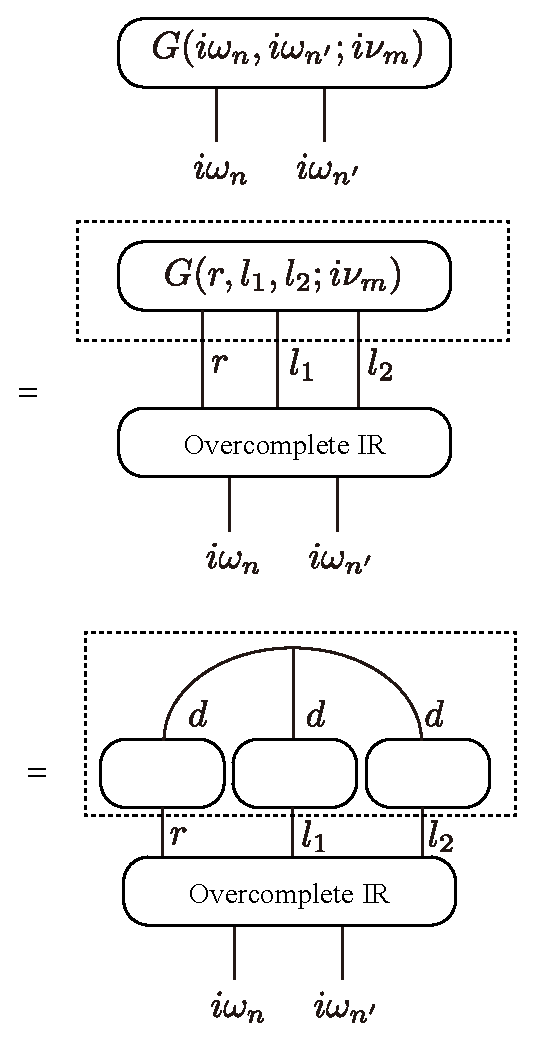
\includegraphics[width=.4\textwidth,clip]{tensor_regression.pdf}
	\caption{
		Graphical representation of CP decomposition
	}
	\label{fig:CP}
\end{figure}

\end{document}
